\chapter{Experiments and Results}\label{ch:experiments-and-results}

This chapter describes our experiments that evaluate and compare the performance of the methods described above and reports the results. For conciseness, here we refer to the implementations of the ILP-, SAT- and DP-based algorithm as \textsf{ILP}, \textsf{SAT}, and \textsf{DP} respectively.

\section{Data}

To evaluate the implementation, we require a set of graphs which will be provided as input to the algorithm. To acquire them, we used the online database The House of Graphs~\cite{HoG} that contains interesting graphs. We decided to conduct experiments on these graphs, as they are most likely to be typical targets of the algorithms. In this work, we experimented with a small subset of all those graphs.

The problem of computing the local circular crossing number is NP-hard. Consequently, the resources required by all implemented algorithms grow exponentially with the input size. To be able to perform the experiments, we had to limit the size of the graphs. We have done this by picking only graphs with at most \(10\) vertices. This constraint leaves plenty of graphs to experiment with while significantly limiting the computational resources. Also, as we designed the implementation only for connected graphs, we filtered out unconnected graphs.

This query resulted in \(2007\) different graphs. Among them \(1326\) are biconnected and \(681\) are not.


\section{Experiment setup}

All experiments described below were conducted on a virtual cloud server provided by Amazon Web Services. The hardware available was limited to a single core of an AWS Graviton4 Processor and 2GiB of random access memory. As an operating system, we used Linux.

For each experiment, we chose a set of graphs, a set of methods, and a set of configurations. We constructed all possible triplets of these parameters. For each one of them, we compute the local circular crossing number of the given graph using the specified method in a given configuration. Apart from recording the number itself, we also track the time required by the corresponding algorithm, which does not include the time required to start up and parse the graph, as it is part of any algorithm. Unfortunately, some methods require an unreasonable amount of time to calculate the result for some graphs. To mitigate this, we limit the execution time to \(10\) minutes for each triplet, indicating the outcome in the results.

We save the results of each experiment in \textsc{csv} format. For each entry, we specify the Graphviz representation of the graph, the configuration, the method, and the execution results. The latter includes the local circular crossing number, the time required to compute it and whether the algorithm succeeded or not.

Apart from reporting, we also use the results obtained by all experiments to cross-validate the correctness of the implementations. Since no algorithm has been previously implemented for recognising outer \(k\)-planar graph, we do not have a reliable source to provide the correct local circular crossing numbers for test graphs. This cross-validation acts as a primary method for testing the implemented algorithm, with the only other one being manual verification of the returned drawing for small instances.

It is worth noting that the Gurobi optimiser supports multithreading. However, to make the comparison of the algorithms fair, we limited it to a single thread.

\begin{figure}[tbh]
    \centering
    \subfloat[\textsf{ILP}]{
        \label{fig:bctree-results:ilp}
        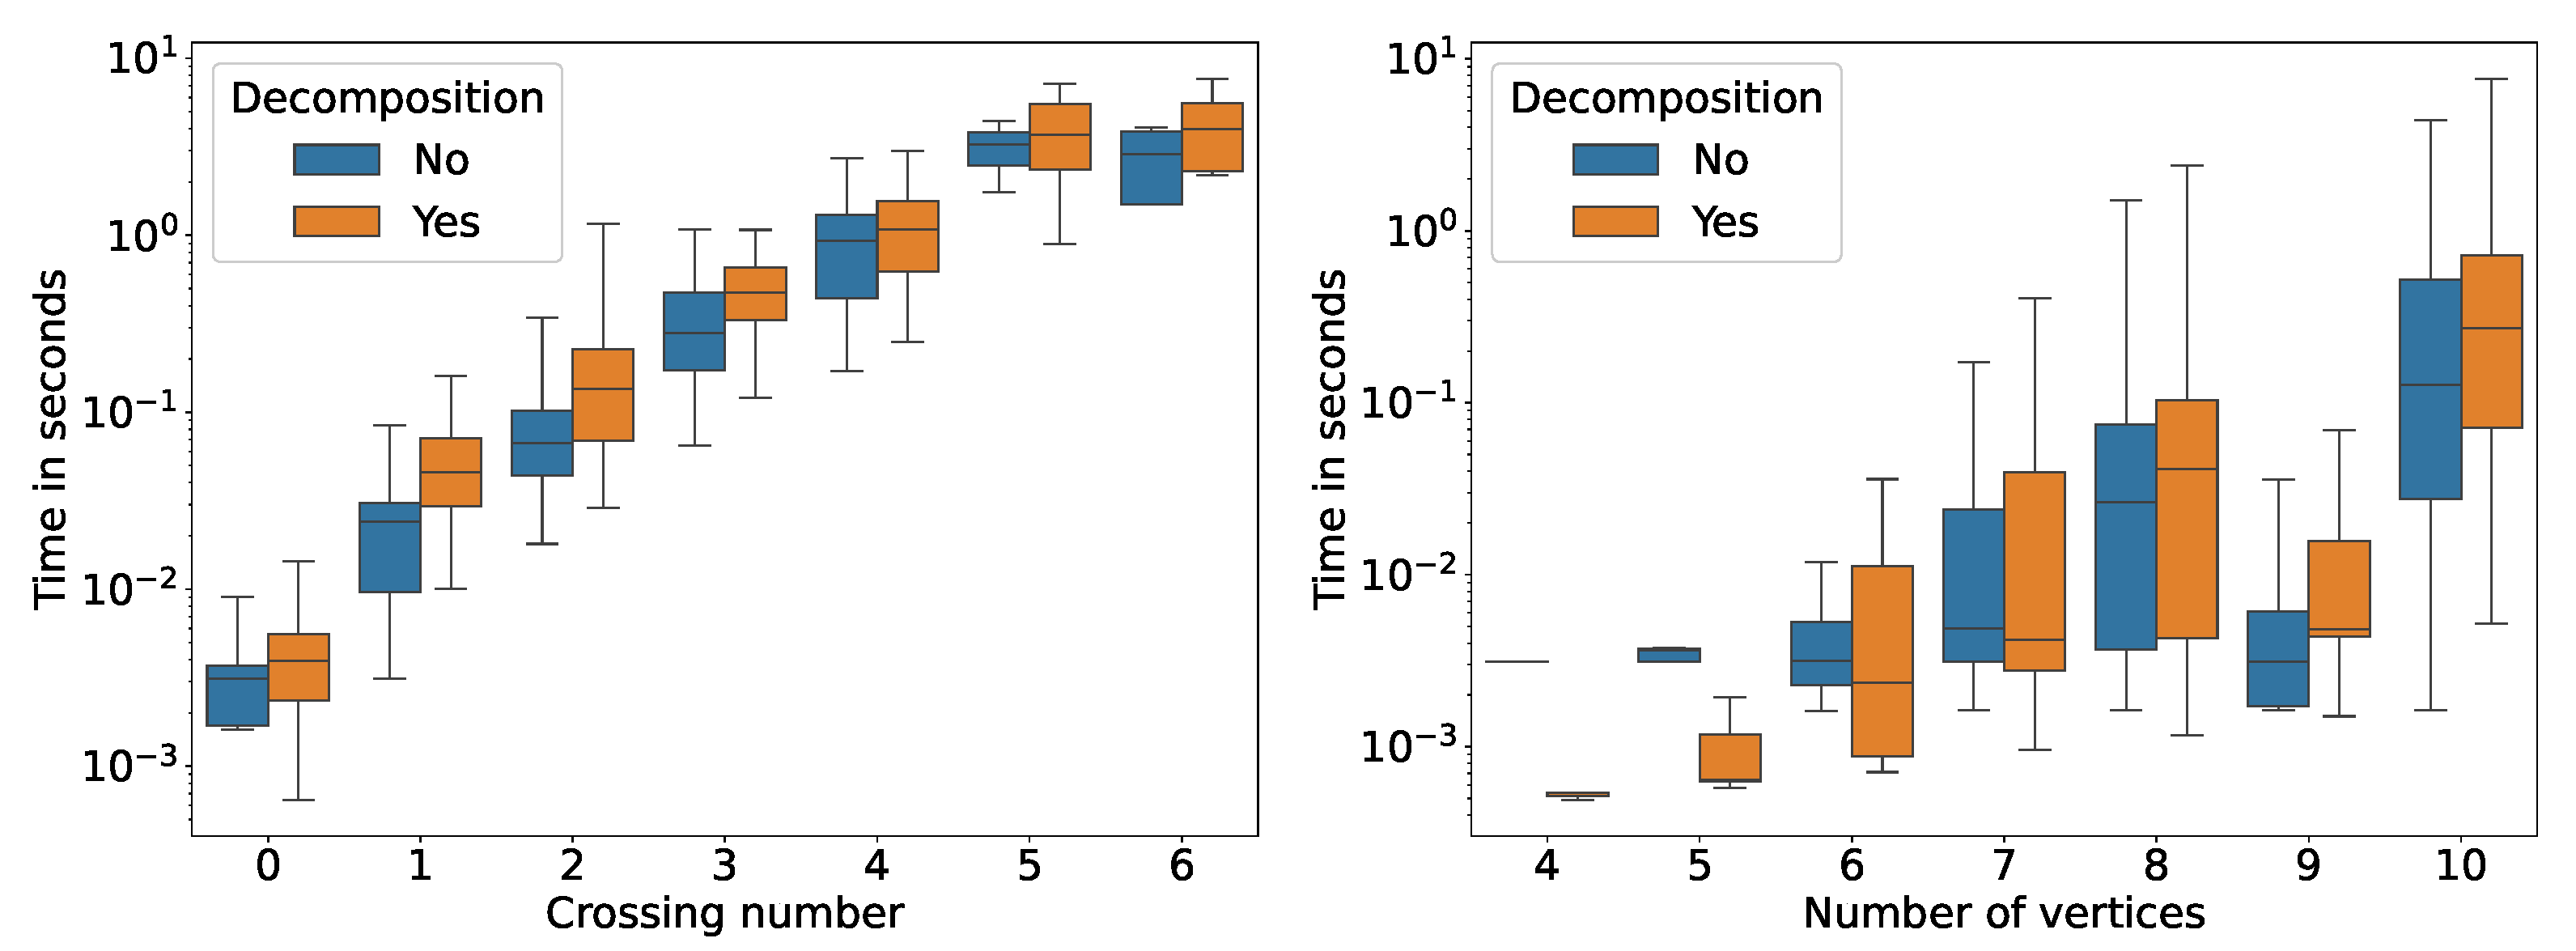
\includegraphics[width=.97\textwidth]{experiments/bctree_ilp}
    } \hfill
    \subfloat[\textsf{SAT}]{
        \label{fig:bctree-results:sat}
        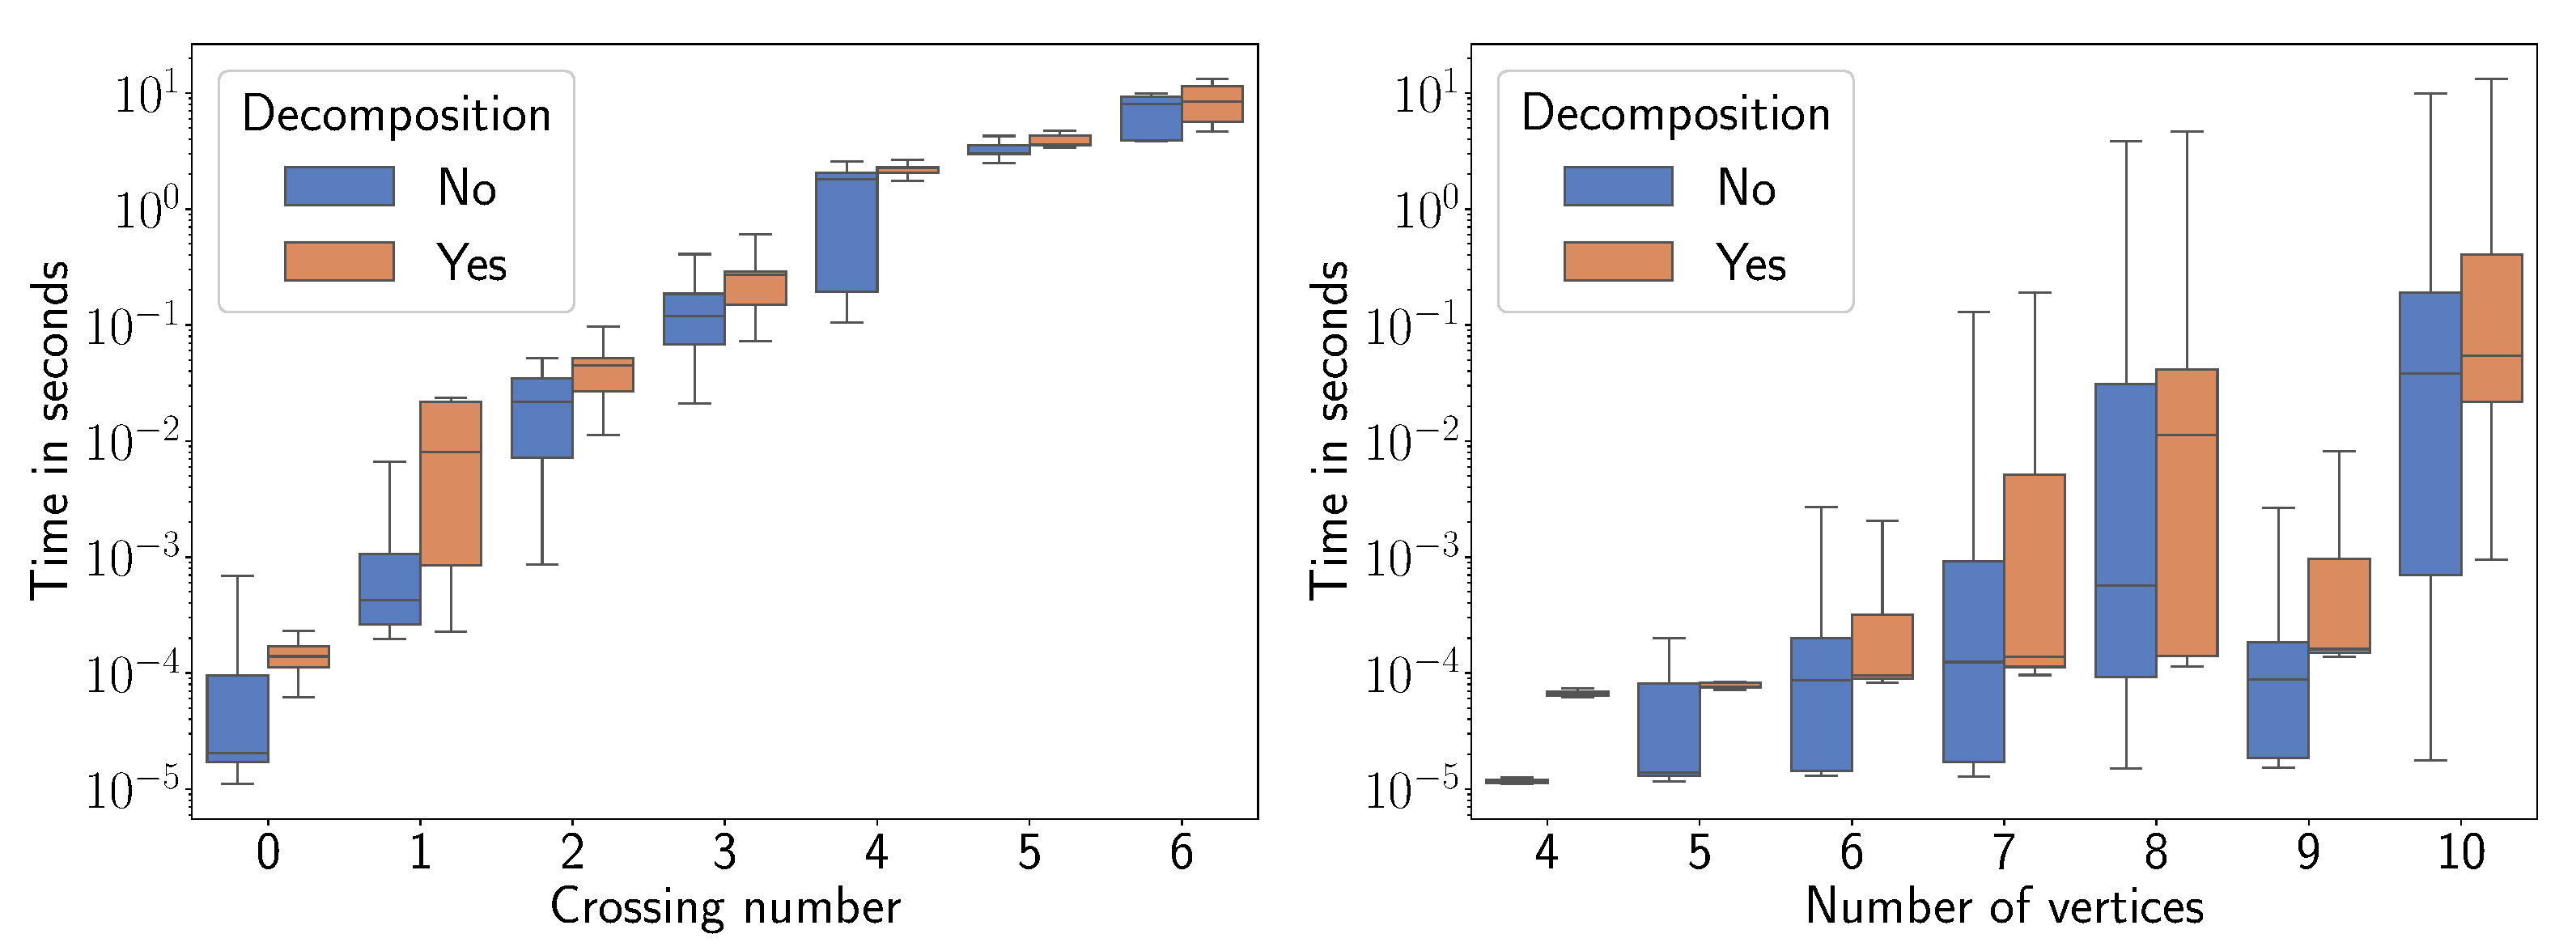
\includegraphics[width=.97\textwidth]{experiments/bctree_sat}
    } \hfill
    \subfloat[\textsf{DP}]{
        \label{fig:bctree-results:okp}
        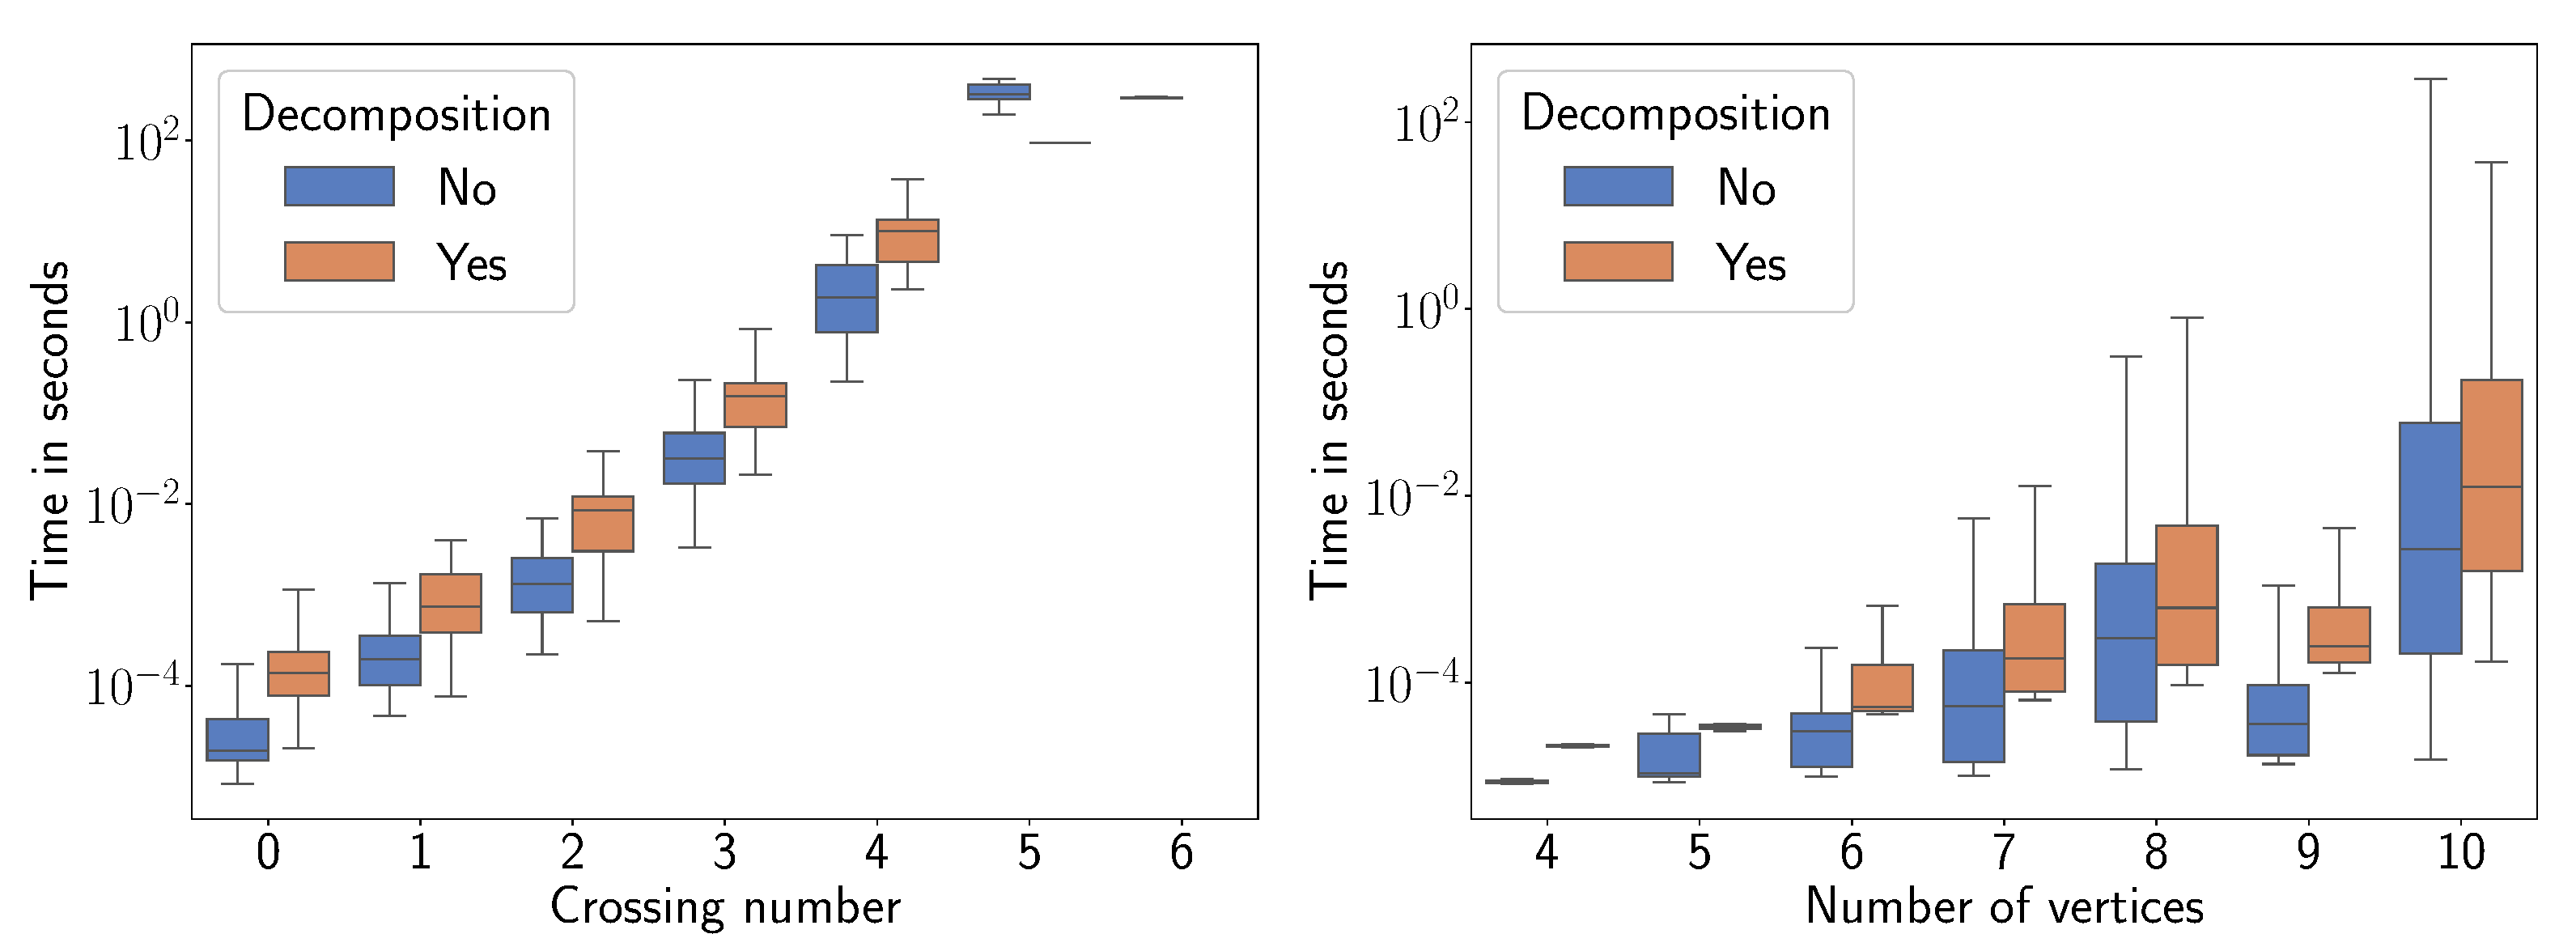
\includegraphics[width=.97\textwidth]{experiments/bctree_okp}
    }
    \caption{Results of the experiment, demonstrating the influence of biconnected decomposition on the running time of \textsf{ILP} , \textsf{SAT} and \textsf{DP}.}
    \label{fig:bctree-results}
\end{figure}

\section{Biconnected decomposition}

The first experiment we considered was comparing the performance of the algorithms with and without bicomponent decomposition. Here, we used only non-biconnected graphs from the dataset to show the difference between the two configurations. We ran this for all three methods. The results are presented in the~\Cref{fig:bctree-results}.

The results prove that using decomposition indeed boosts performance for almost all methods and graphs. The only exceptions are small graphs for \textsf{ILP}, for which the cost of initialising multiple environments outweighs the cost of decoupling the problem.

As we demonstrated in this experiment, the non-biconnectivity of the graphs artificially decreases the complexity of the recognition task, as each one of them requires multiple times fewer resources compared to equally sized biconnected graphs. Thus, in the following experiments, we consider only biconnected graphs to exclude this source of noise from the results.


\section{Comparison of the algorithms}

In this experiment, we compared the performance of the algorithms. We grouped results by crossing numbers and the algorithm used for solving and displayed in~\Cref{fig:methods}. Due to the complexity of the problem, some runs ran out of allocated resources. So, to display the results, we used only the measurements from runs that successfully found the minimal crossing number. As a result, starting from \(k = 6\), boxes for \textsf{SAT} and \textsf{DP} depict fewer runs compared to \textsf{ILP} as they required more resources for some graphs than were available.

\begin{figure}[tbh]
    \centering
    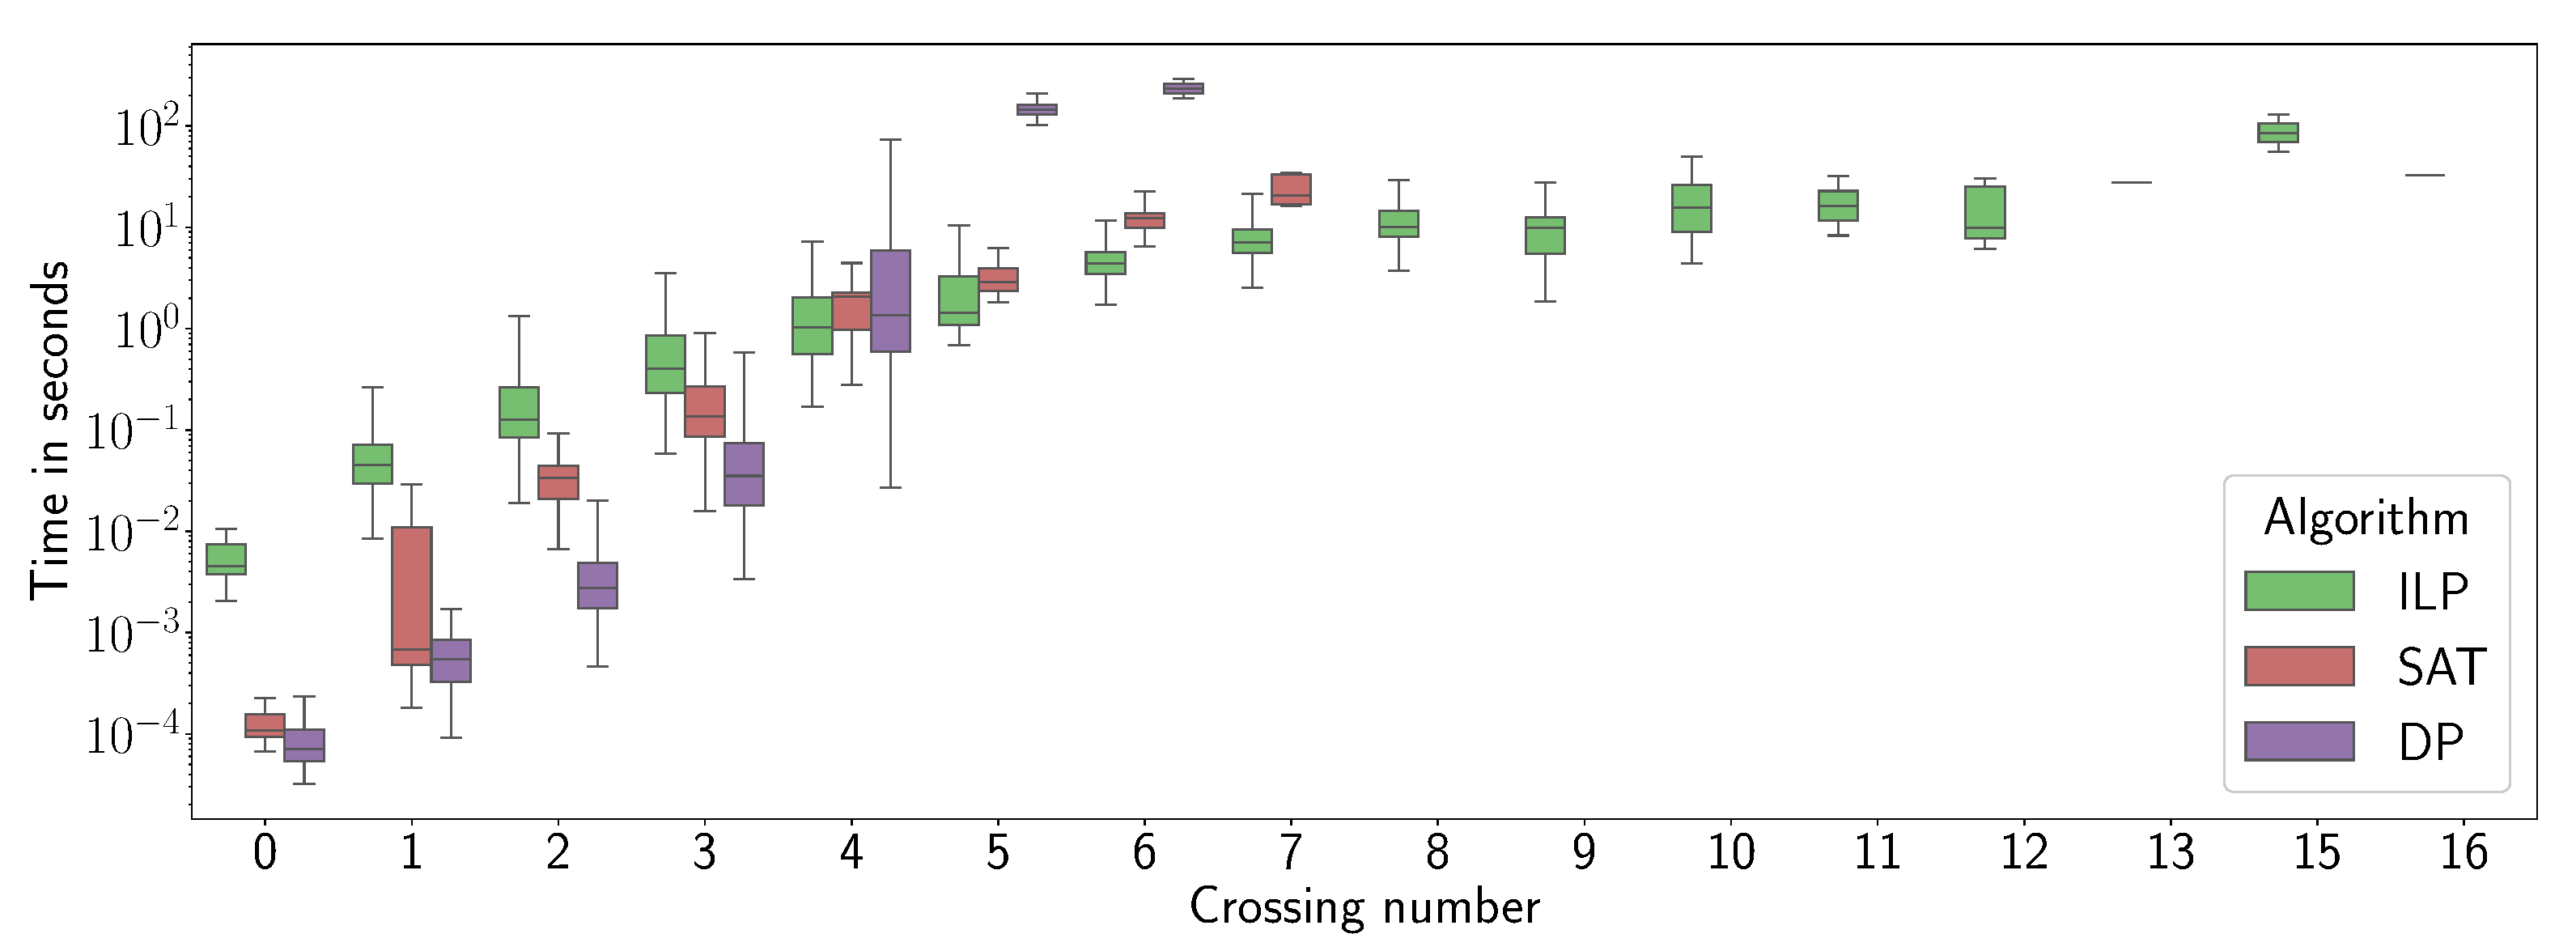
\includegraphics[width=\textwidth]{experiments/methods}
    \caption{Comparison of running times of different algorithms for graphs with different crossing numbers.}
    \label{fig:methods}
\end{figure}

\textsf{SAT} and \textsf{DP}, however, were limited primarily by different factors. Unlike \textsf{ILP}, encoding in \textsf{SAT} contains an exponential number of clauses in terms of local circular crossing number. As a result, the solver ran out of allocated memory for \(185\) out of \(1326\) biconnected graphs. Similarly, \textsf{DP} ran out of memory \(16\) times. However, the bigger limiting factor for this algorithm is time, as \(317\) runs exceeded the 10-minute time limit imposed on each one. All other runs finished successfully.

The results show that the time required by both \textsf{SAT} and \textsf{DP} grows much faster than the time required by \textsf{ILP}. The latter requires each instance to set up an environment for the graphs. With smaller crossing numbers, these costs outweigh the solver's speed. However, for instances with bigger \(k\), the time required for setup is negligible.

\begin{figure}[tbh]
    \centering
    \subfloat[\(k = 2\)]{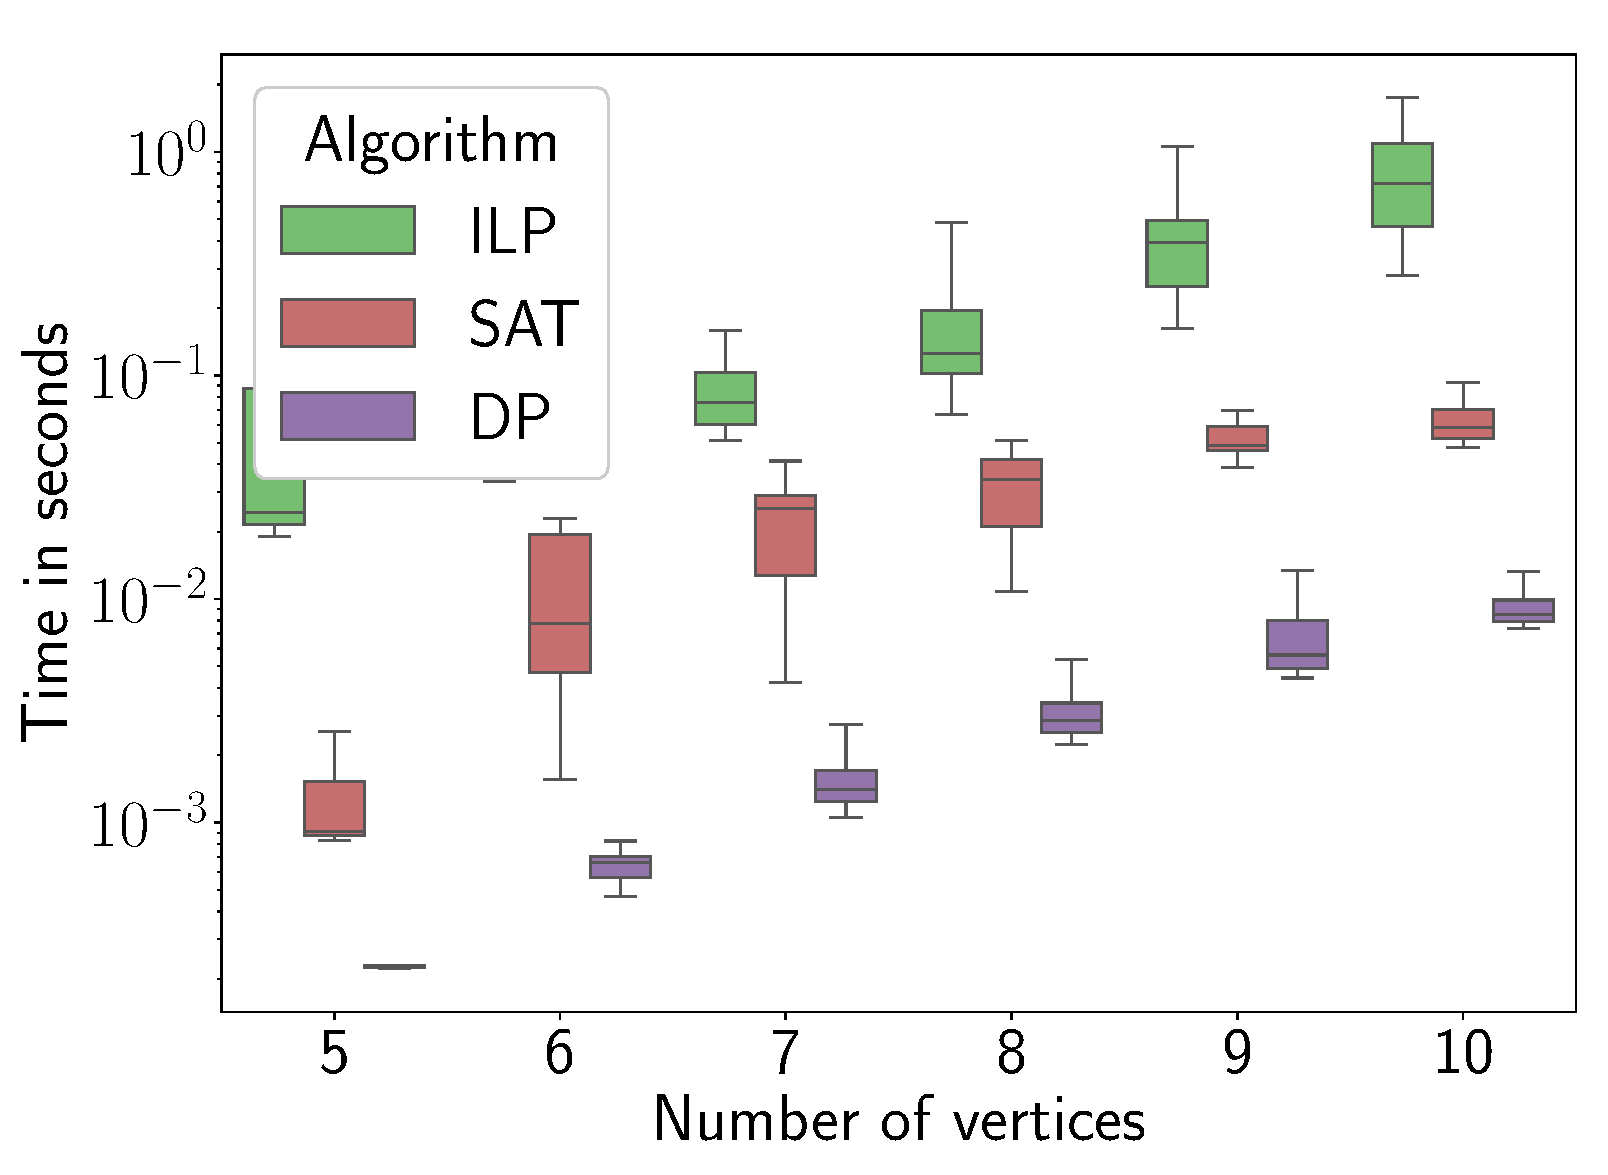
\includegraphics[width=.48\textwidth]{experiments/method_2}} \hfill
    \subfloat[\(k = 3\)]{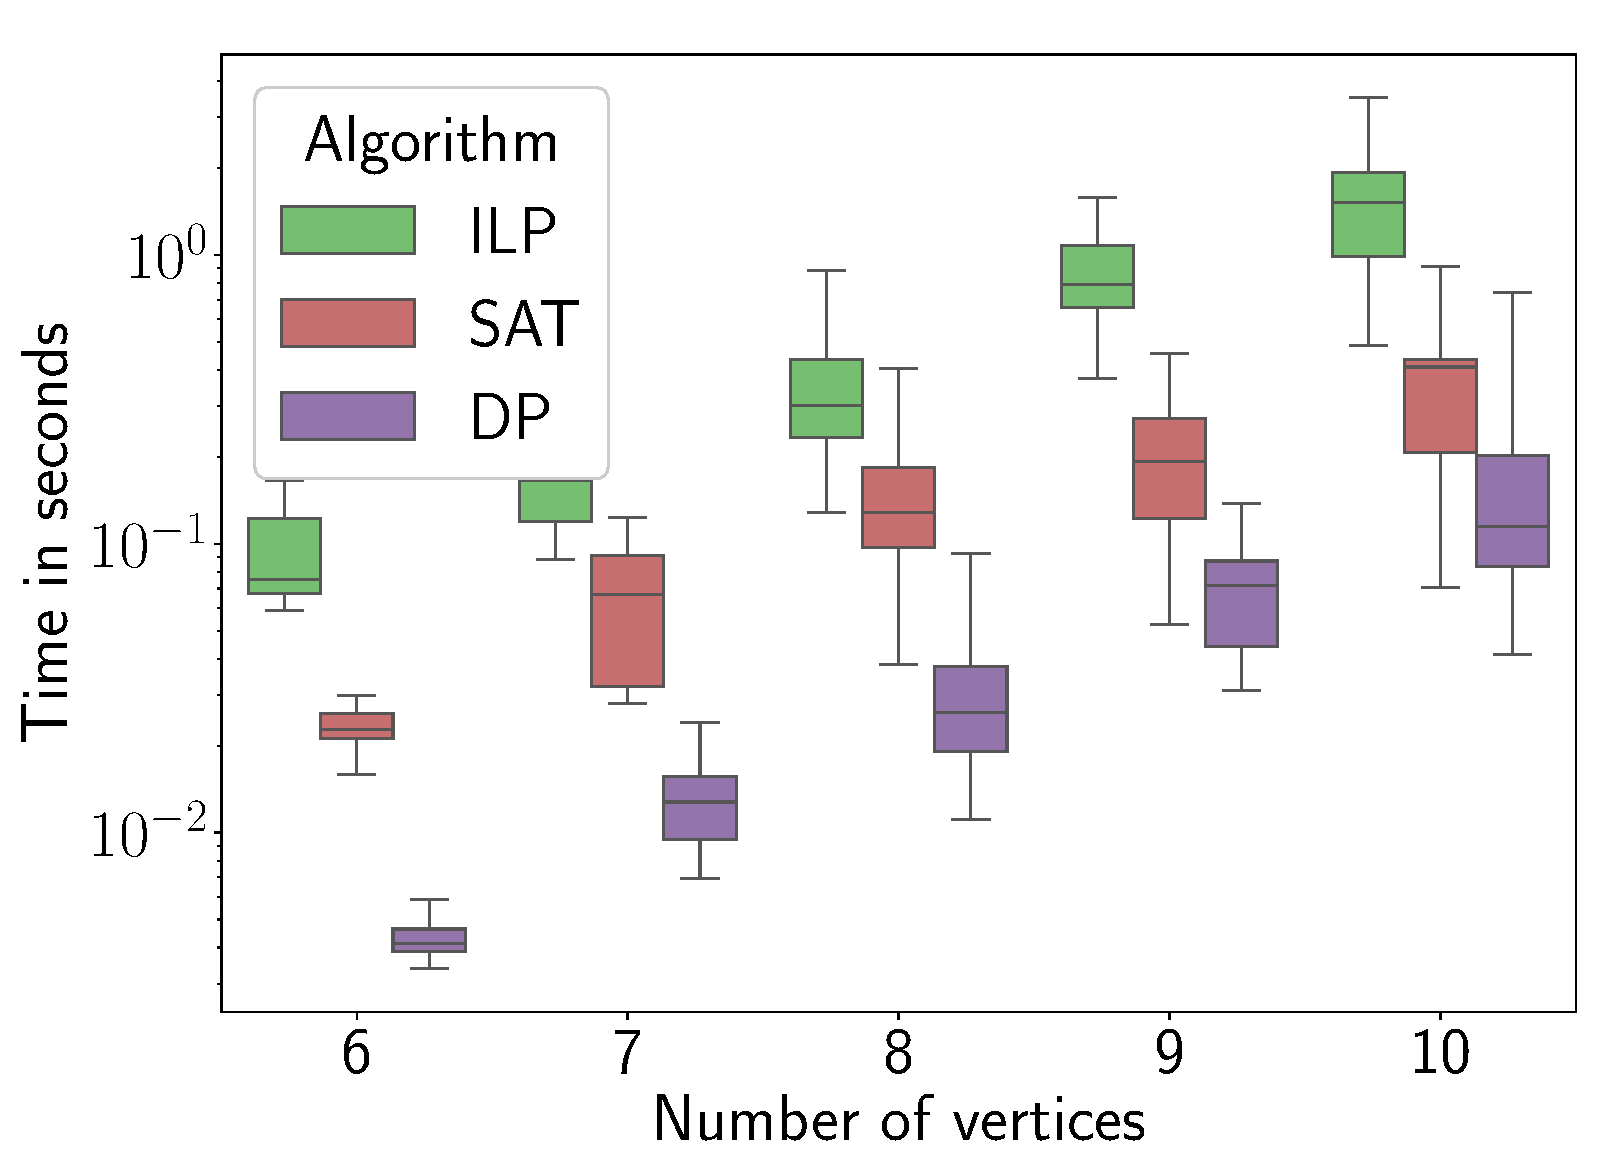
\includegraphics[width=.48\textwidth]{experiments/method_3}} \hfill
    \subfloat[\(k = 4\)]{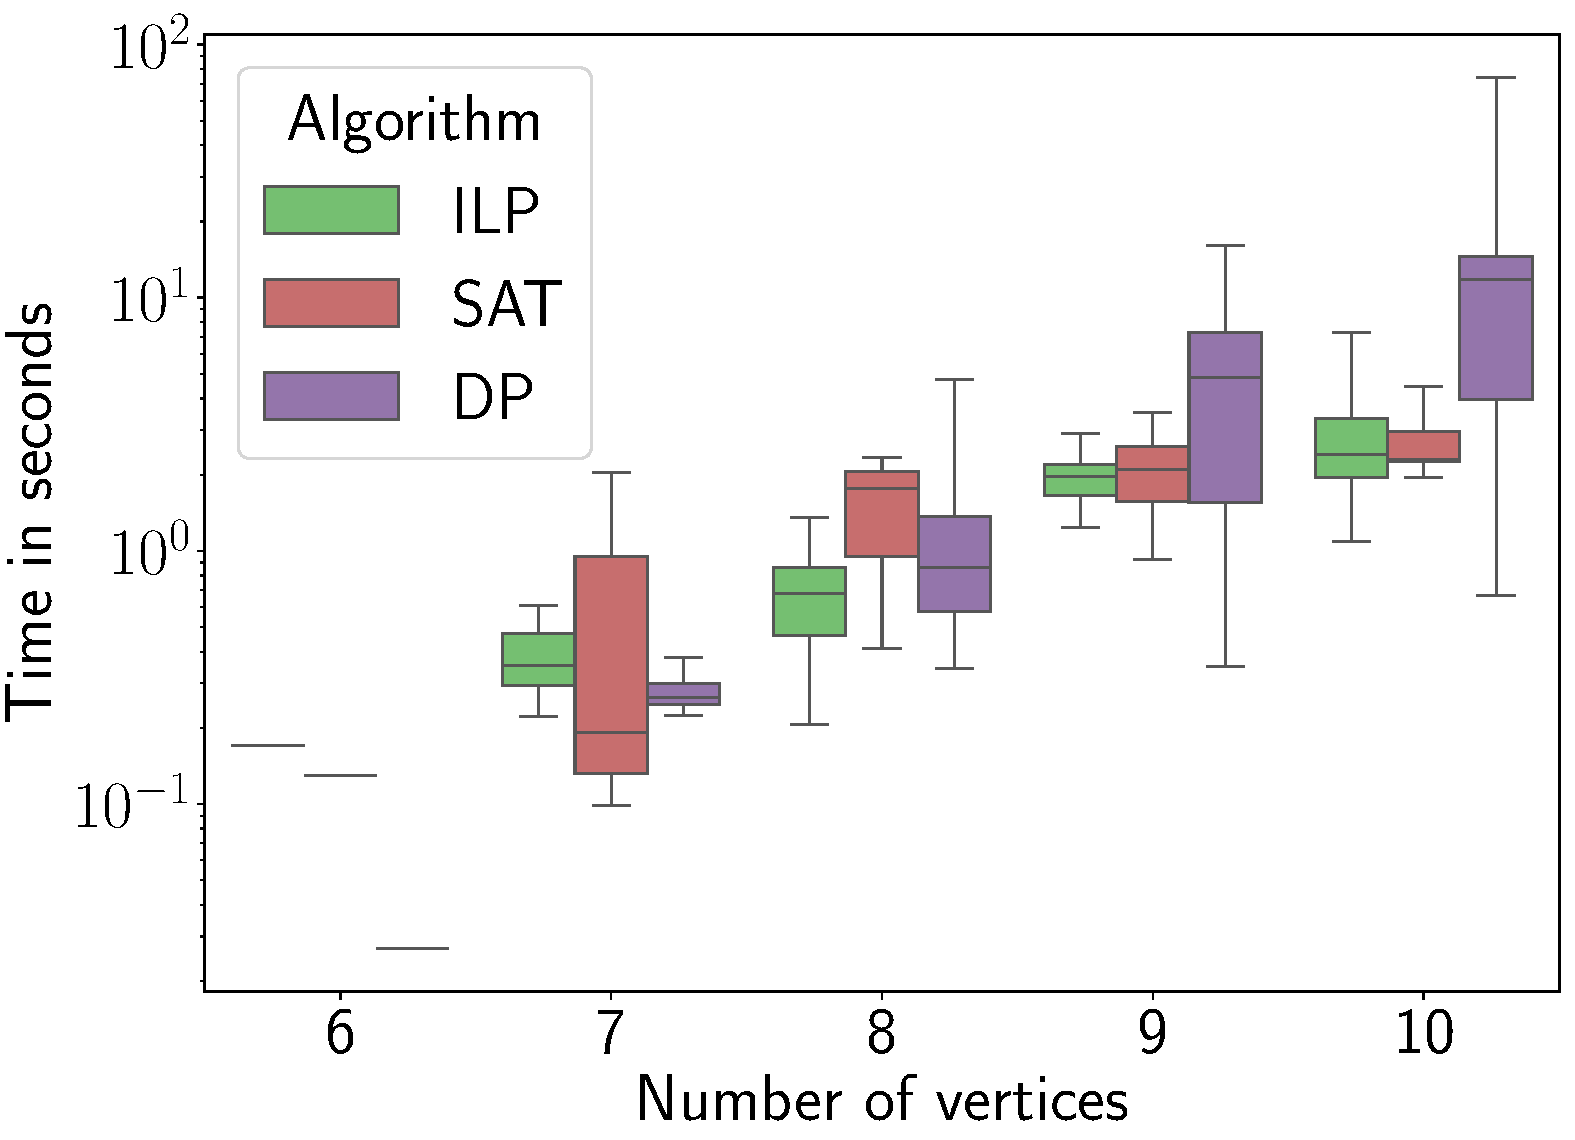
\includegraphics[width=.48\textwidth]{experiments/method_4}} \hfill
    \subfloat[\(k = 5\)]{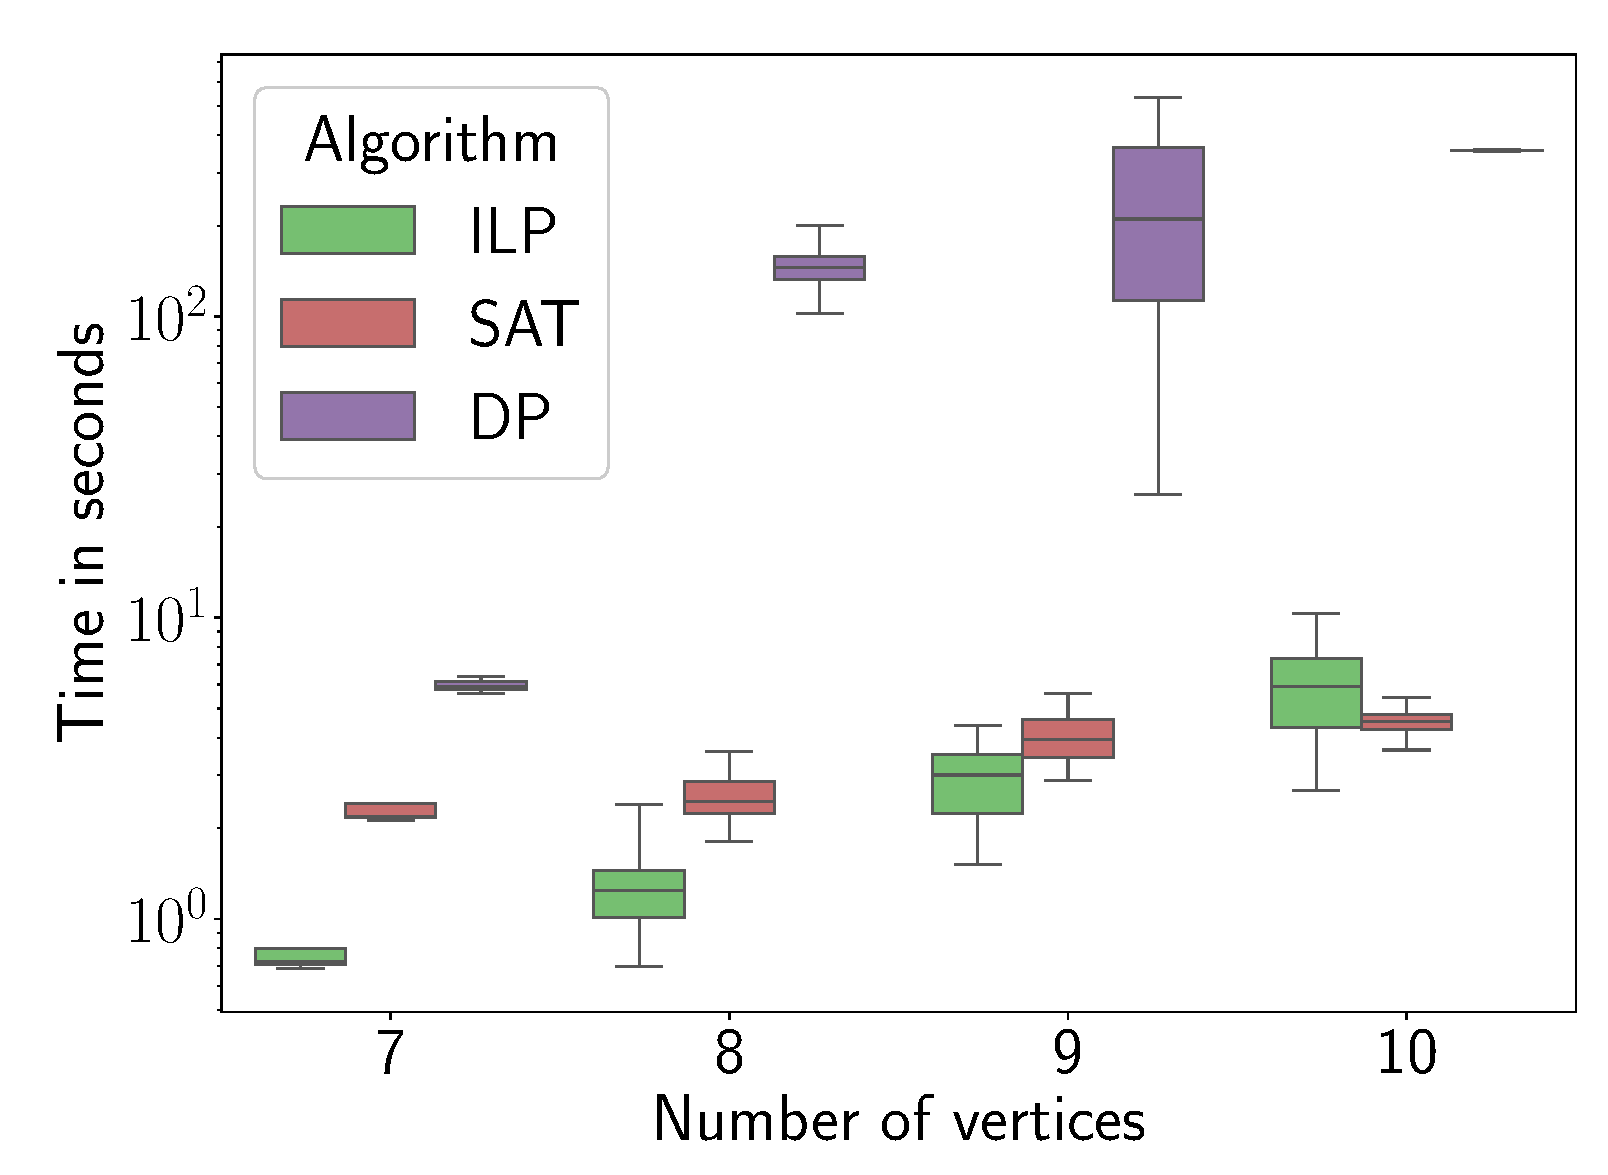
\includegraphics[width=.48\textwidth]{experiments/method_5}} \hfill
    \caption{Comparison of running times required by algorithms to recognise outer \(k\)-planar graphs for various values of \(k\).}
    \label{fig:methods-vertices}
\end{figure}

As the algorithm's running time depends not only on crossing numbers but also on the size of the graph, we can represent the results more accurately by grouping them by both the crossing number and the number of vertices. To demonstrate this dependency, in~\Cref{fig:methods-vertices}, we created a plot for each crossing number represented by at least \(150\) graphs. These plots show that, for \(k \in \{2, 3\}\), \textsf{DP} and \textsf{SAT} are consistently the two fastest methods, with the former being faster than the latter. However, starting from \(k = 4\) and graphs with at least \(9\) vertices, \textsf{ILP} outperforms the other two methods. Most importantly, these results agree with the ones displayed in~\Cref{fig:methods}, which aggregate them for each value \(k\).


\section{Optimisation benchmark}

The last experiment we considered is the comparison of optimisations we discussed for \textsf{ILP} and \textsf{SAT} in~\Cref{sec:optimisations}. For \textsf{ILP}, we ran four configurations for each biconnected graph using none, one, or both optimisations. For \textsf{SAT}, we used two configurations with and without optimisation. The results are presented in~\Cref{fig:optimisation:ilp} and~\Cref{fig:optimisation:sat} respectively.

\begin{figure}[tbh]
    \centering
    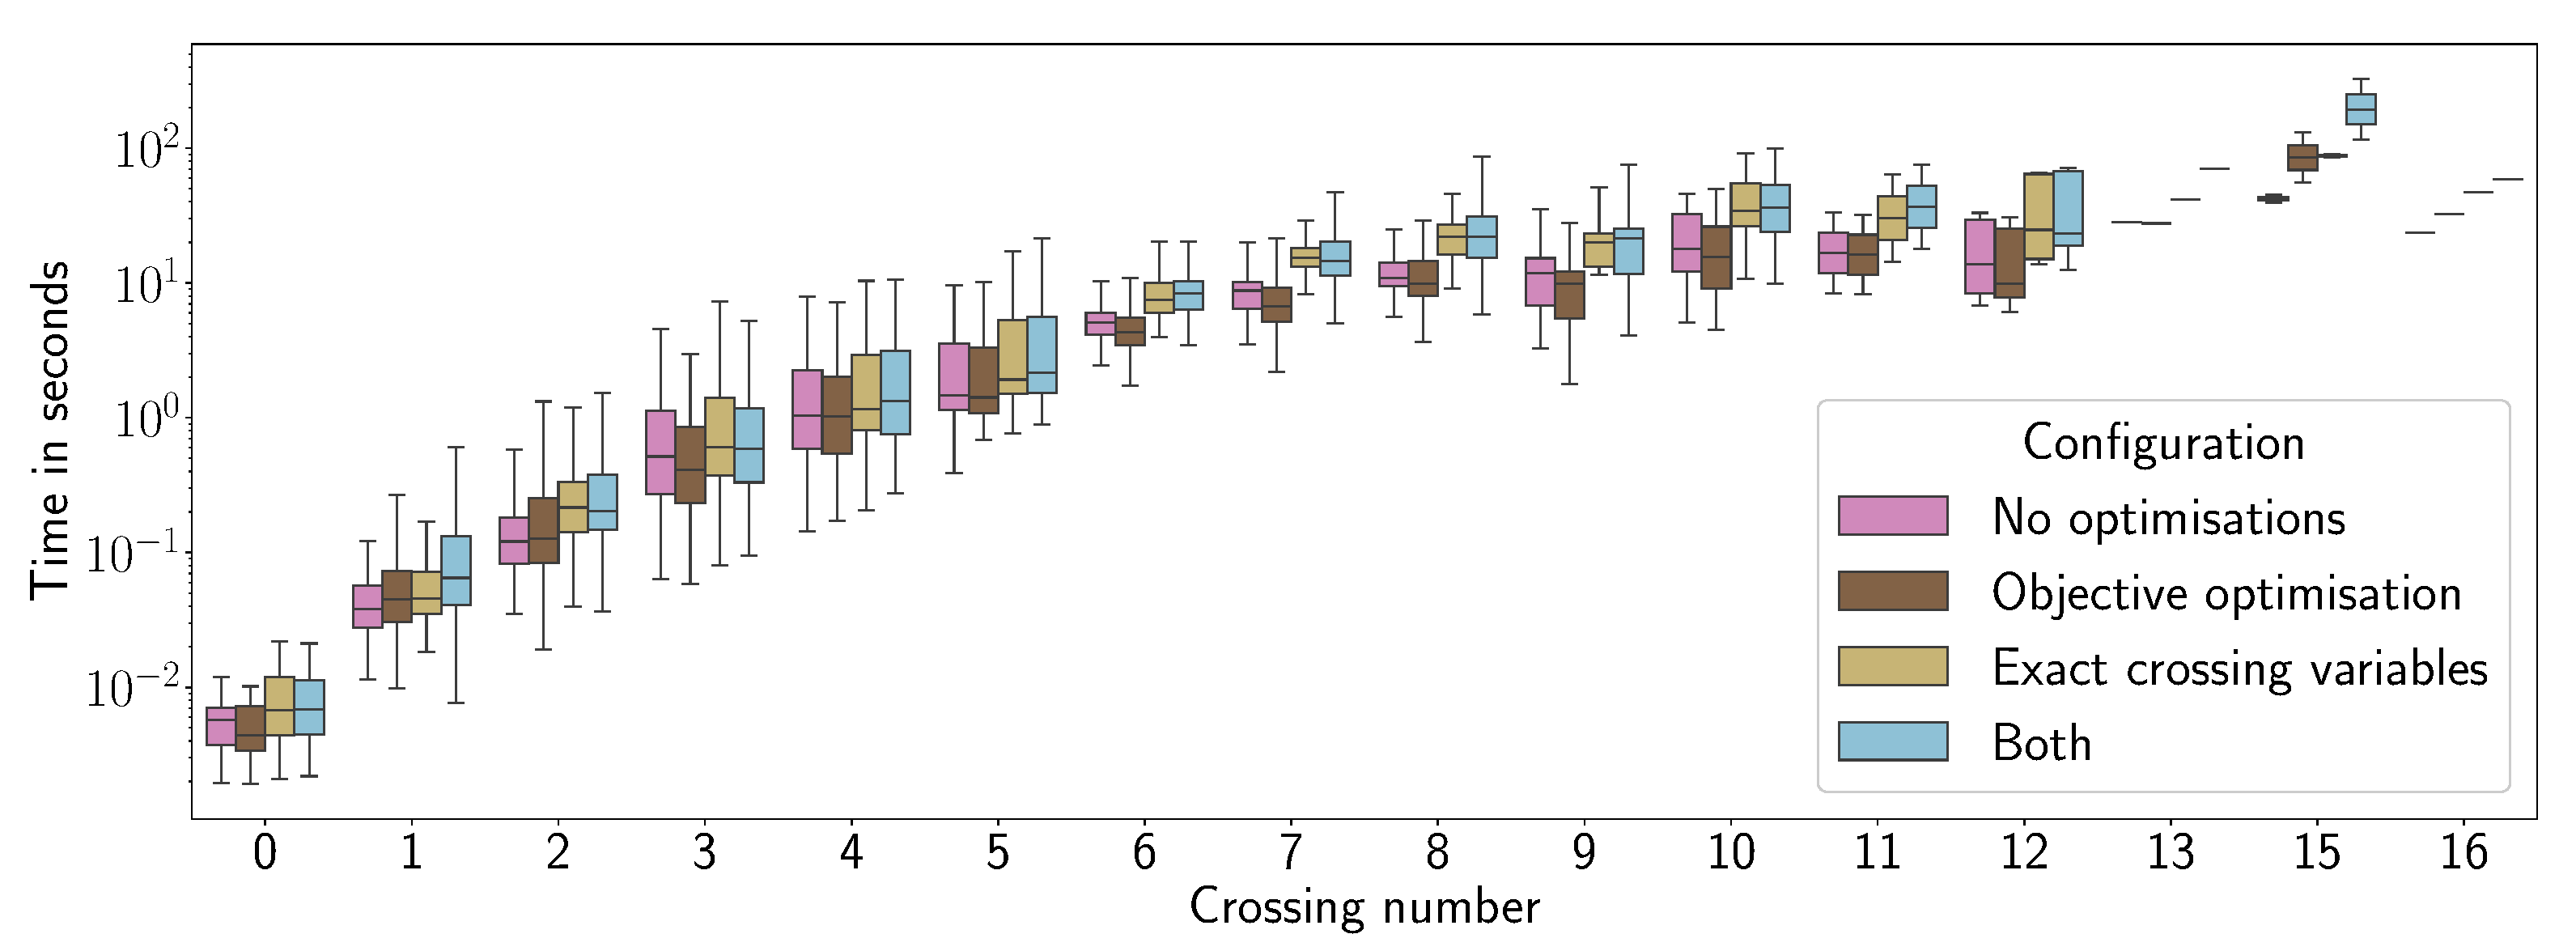
\includegraphics[width=\textwidth]{experiments/ilp}
    \caption{Comparison of different configurations for \textsf{ILP}.}
    \label{fig:optimisation:ilp}
\end{figure}

\begin{figure}[tbh]
    \centering
    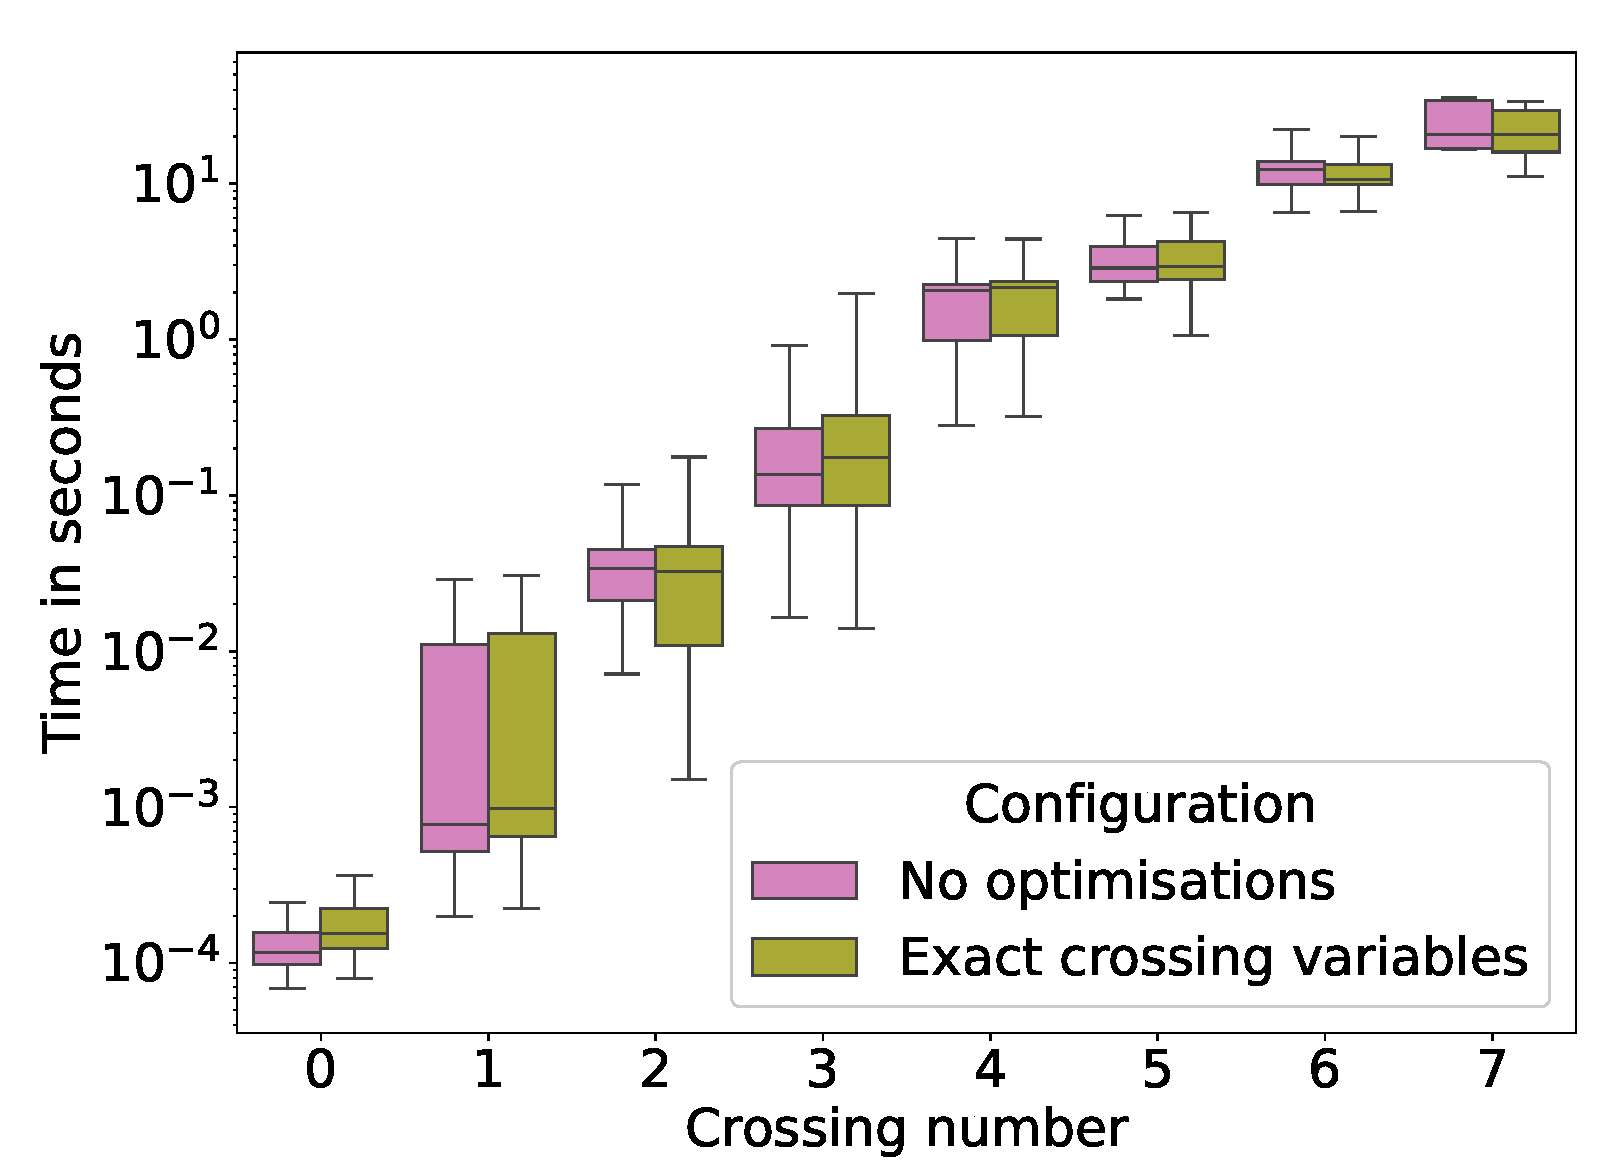
\includegraphics[width=0.47\textwidth]{experiments/sat}
    \caption{Comparison of different configurations for \textsf{SAT}.}
    \label{fig:optimisation:sat}
\end{figure}

In the first plot, we can clearly see that adding additional constraints to enforce the exact value for each crossing variable degrades the performance. For \textsf{SAT}, however, this change does not influence this much. We can see a slight rise in execution time, but the difference is within the margin of error. Here, the difference may be caused by the algorithm writing down the required additional constraints, not the SAT solver.

The objective optimisation for \textsf{ILP}, which includes an extra term in the objective function, makes small but still an improvement. As a result, we consider the algorithm that includes this optimisation to be the most efficient \textsf{ILP}. Thus, we have used this configuration for all other experiments. For \textsf{SAT}, we used a configuration that did not include optimisation.
